% ============================================================================
%  Beautified Is Not Forged -- paper v6b (2026-10-17), anonymous submission version. Revision of main_v6.tex: the full-data model
%  trained with the forgery head only is the first (detection-reference) row of every detection table, the full model (three
%  classes + operations) is reported beside it, second seeds and identity intervals added, rounding aligned with FINDINGS.md.
%  Changes and sources: V6B_CHANGES.md. Tables: make_tables_v6b.py (tab_v6b_*, fig_accuse_v6b), make_tables_v6.py (tab_v6_*),
%  make_tables_v5.py (tab_v5_*), make_tables_cgd.py; teaser make_fig_teaser_v6b.py. Supplement: supplement_v6b.tex.
% ============================================================================
\documentclass[conference]{IEEEtran}
\IEEEoverridecommandlockouts
\usepackage{fontspec}
\setmainfont{texgyretermes}[Extension=.otf,UprightFont=*-regular,BoldFont=*-bold,ItalicFont=*-italic,BoldItalicFont=*-bolditalic]
\usepackage{cite}
\usepackage{amsmath,amssymb,amsfonts}
\usepackage{graphicx}
\usepackage{booktabs}
\usepackage{array}
\usepackage{adjustbox}
\usepackage{xcolor}
\usepackage{url}
\usepackage{capt-of}
\usepackage{xr-hyper}
\usepackage[hidelinks]{hyperref}
\newcommand{\ours}{\textsc{Ours}}
\newcommand{\oursB}{\textsc{Ours}, forgery head only}
\newcommand{\oursF}{\textsc{Ours}, full model}
\externaldocument[S-]{supplement_v7}
\graphicspath{{figs/}}
\renewcommand{\dbltopfraction}{0.95}
\renewcommand{\topfraction}{0.95}
\renewcommand{\textfraction}{0.05}
\raggedbottom

\begin{document}

\title{Beautified Is Not Forged: Skin Smoothing Is a Shared Shortcut of Face-Forgery Detectors}

\author{\IEEEauthorblockN{Anonymous submission}}

\IEEEaftertitletext{\vspace{-0.6\baselineskip}\begin{center}
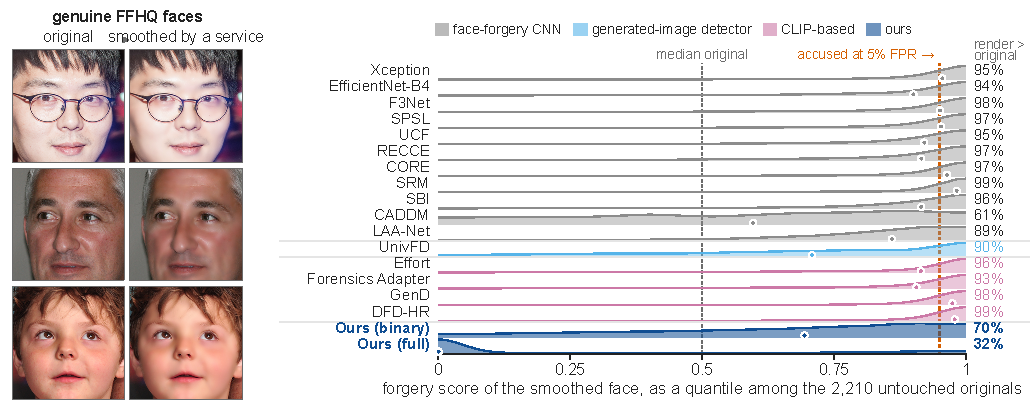
\includegraphics[width=0.98\textwidth]{fig_teaser_v7}
\captionof{figure}{Every published detector scores a skin-smoothed genuine face as more forged than the same face untouched.
Left: three FFHQ photographs and their renders by a commercial retouching service (skin smoothing, strongest level). Right: for
sixteen published detectors and two of ours, where the smoothed render falls among the 2,210 untouched originals (quantile of
the forgery score; 0.95 is the threshold that accuses 5\% of originals), with the share of pairs in which the render scores
above its own original at the right. NPR is omitted: its scores saturate on this source. Families: face-forgery CNNs,
generated-image detector, CLIP-based detectors, ours.}\label{fig:teaser}
\end{center}\vspace{0.1\baselineskip}}
\maketitle

\begin{abstract}
A genuine face that was beautified by a camera app, an AR filter or a retouching service still shows the same person doing
the same thing, but a forgery detector may not treat it that way. We score seventeen published detectors on six
beautification sources with one rule and find one failure shared by all of them: a skin-smoothed genuine face is scored as
more forged than the same face untouched, in 89--99\% of pairs for fifteen detectors, and smoothing the skin alone is enough.
We then show where the cue comes from. With architecture, data and recipe fixed, the class that receives smoothed views
during training sets the sign of the error: views on genuine faces only let nearly every smoothed forgery through, views on
forged faces only accuse smoothed genuine faces, and views on both sit in between. From this we derive a training rule,
smoothing-invariant consistency (SIC): one smoothing operator drawn identically for both classes and a penalty on the change
of the forgery logit under it. At a penalty weight of 0.1, SIC lowers the false alarm on skin-smoothed genuine faces from 85\% to 4\% while untreated
video AUC on Celeb-DF-v2 moves from 0.956 to 0.930. No setting removes the cue for free: raising the decision threshold with a
smoothing estimate clears the genuine faces and lets every smoothed forgery through, and the penalty weight trades untreated
detection against the miss on smoothed forgeries. We release the six sources, the scorer and the paired reader as a benchmark.
\end{abstract}

% ----------------------------------------------------------------------------
\section{Introduction}
Forgery detectors are used for content moderation, remote identity checks and fact-checking. In each setting a genuine face
called fake accuses a real person, and a forgery called real is let through. A large share of the genuine faces reaching
such a detector were beautified before upload: skin smoothing, whitening, eye enlargement and face slimming are default
options in camera apps and retouching services, and colour presets ship with every photo-sharing app. Beautification edits
the pixels a detector inspects but changes neither who is shown nor what the person does.

Prior work measured the effect of beautification on at most six detectors and in one direction at a
time~\cite{libourel2024,saeed2025,concas2025}. We ask three questions. Does the effect hold across the detector families
in use today? Where does it come from? Can it be removed without giving up detection?

\paragraph{Finding.} We score seventeen published detectors, eleven CNN detectors, four CLIP-based detectors and two
generated-image detectors, on six beautification sources with one rule that counts both errors (Fig.~\ref{fig:teaser}).
The failure shared by all of them is skin smoothing: a smoothed genuine face is scored as more forged than the same face
untouched in nearly every pair, smoothing the skin alone with the background untouched suffices, and for the CLIP detectors
the forgery logit grows with the smoothing strength. A radial vignette alone does not produce the shift.

\paragraph{Cause.} We hold architecture, data and recipe fixed and vary only which class receives smoothed views during
training (Fig.~\ref{fig:exposure}). The class that sees smoothing sets the sign of the error. Views on genuine faces only teach that smoothed means genuine, and a
forger who smooths the forgery is let through. Views on forged faces only teach the opposite. Views on both classes, drawn
from the same operator, sit in between. This is shortcut learning~\cite{geirhos2020} under class-dependent
augmentation~\cite{balestriero2022}; Ricker et al.~\cite{ricker2026biasid} observed the same sign flip for JPEG in
generated-image detection with one-class training, and we measure the full design, with the both-classes arm, for skin
smoothing in face-forgery detection.

\paragraph{Method.} The cause suggests the fix. Smoothing-invariant consistency (SIC) draws one smoothing operator
identically for every training item and penalises the change of the forgery logit under it (Fig.~\ref{fig:arch}). The
model keeps its three-way output and four operation scores; only the forgery logit is constrained. At a weight of 0.1 the
false alarm on skin-smoothed genuine faces falls from 85\% to 4\% and untreated Celeb-DF-v2 video AUC from 0.956 to 0.930
(two seeds). The family traces a three-way trade-off between that false alarm, the miss on smoothed forgeries and untreated
detection, and a threshold rule, which we also test, cannot reach a better point.

Our contributions are:
\begin{itemize}
\item A two-sided measurement of seventeen detectors on six beautification sources under one rule, read pair by pair where
originals exist, with a skin-only smoothing test and a dose-response test that isolate the shared cue.
\item A controlled exposure study in which the class receiving smoothed views decides whether the detector accuses or lets
forgeries through, including an evasion route opened by genuine-only views.
\item SIC, a training rule that removes the cue at a measured cost, evaluated on pre-registered bars with two seeds, a
$\lambda=0$ control and a blur ablation; the finding that no threshold rule separates smoothed genuine from smoothed forged
faces for any of the detectors; and the released benchmark.
\end{itemize}

% ----------------------------------------------------------------------------
\section{Related Work}
\textbf{Beautification and forgery detection.} Libourel et al.~\cite{libourel2024} released Celeb-DF-B and report video AUC
drops for three detectors under app presets; Saeed et al.~\cite{saeed2025} show that face enhancement lets deepfakes evade six
detectors (they measure misses only) and fine-tune Xception on enhanced data without stating which class was enhanced; Concas et al.~\cite{concas2025} apply smoothing filters at test time to genuine, forged or both test images and report both
errors for two CNNs. None scores detectors by a common rule or trains against the edit with a class-controlled design. On smartphone
photographs the false-alarm rate of a generated-image detector is set by where its threshold was
calibrated~\cite{laionmobile2026}. OpenFilter~\cite{openfilter2022} renders Instagram AR filters onto FairFace and LFW.
Retouching detection and restoration~\cite{bharati2016,jain2018,wang2019photoshop,
retouchingffhq,frrffusion,mofrr,reface} have no forgery class; Liu et al.~\cite{miea2026} attribute forgery and beautification
tools in a closed set. Perturbation benchmarks for forgery detection~\cite{deeperforensics2020,moire2025} and for
classification~\cite{hendrycks2019} treat edits as corruptions of one class.

\textbf{Shortcuts and attacks.} Shortcut learning~\cite{geirhos2020} and group shifts~\cite{sagawa2020} describe a model that
learns a feature correlated with the label; Balestriero et al.~\cite{balestriero2022} show that augmentation and regularisation
act differently per class, and Ricker et al.~\cite{ricker2026biasid} train a generated-image detector with JPEG applied to the
real class only or the fake class only and find that the direction of the resulting error flips; they study scene images and
compression, train neither the both-classes case nor a fix, and do not consider faces or beautification. StatAttack~\cite{statattack2023} and AdvShadow~\cite{advshadow2024} optimise natural appearance
changes so that forgeries pass, Fatima et al.~\cite{fatima2025} train on the worst of random counter-forensic transforms, and
semantic adversarial training exists for classification~\cite{hosseini2018,laidlaw2019,gat2023,ava2021}.

\textbf{Generalisable forgery detection.} Face X-ray~\cite{facexray} and SBI~\cite{sbi} synthesise blending artefacts,
UCF~\cite{ucf} separates common from method-specific features, LSDA~\cite{lsda} augments forgery features in latent space for
cross-method generalisation, Effort, Forensics Adapter, GenD and DFD-HR adapt CLIP ViT-L/14, and CORE~\cite{core} ties the representation of two generic augmentations of a frame (flip, rotation, Gaussian blur, JPEG); we show that the choice of operator and its symmetry across classes, not consistency as such, decide whether smoothing is learnt as a cue (Sec.~\ref{sec:sic}). The alpha-blending
hypothesis~\cite{alphablend2026} holds that frame-based detectors read compositing artefacts, and its authors ensemble a
blending detector with blend-resistant models. DeepfakeBench~\cite{deepfakebench} and DF40~\cite{df40} provide checkpoints and
test sets.

\textbf{Explanations.} Joint detection and segmentation~\cite{nguyen2019multitask,hifinet2023}, attention trained so that
erasing it removes the evidence~\cite{gain}, amortised maskers~\cite{dabkowski2017,phang2020}, DOLOS~\cite{dolos} and
FakeVLM~\cite{fakevlm2025} precede our footprint-supervised maps; our addition is a restoration test against the true footprint.

% ----------------------------------------------------------------------------
\section{Problem and Evaluation Rule}
\label{sec:protocol}
\textbf{Classes.} A face image is \emph{forged} if it shows a person, an expression, a motion or speech that was not captured:
another identity in whole or in part, a reenactment or lip-sync, or a face or a facial feature (eye, nose, mouth) replaced by
new content. It
is \emph{beautified} if its colour, tone, skin texture or the smooth shape of the person's own features were edited after
capture while identity, expression, pose and speech stay those of the capture. The label follows what changed, not the tool: a
retouching service that smooths skin with a neural network beautifies, and a reenactment that keeps the identity forges. The
two attributes are independent, and a beautified forgery is forged. The supplement lists 17 cases near the boundary with their labels. A part of the same person regenerated by inpainting was not captured, so we label it
forged; we have not measured identity or expression preservation for any edit family, so the boundary is stated, not
operationalised.


\textbf{Rule.} A detector should return a forgery score that does not move when a face is beautified; whether a face was
beautified can be reported as a separate attribute, and every detection number reads the forgery score alone. Each detector is
scored by $P(\text{fake})$ with the threshold that accuses 5\% of each source's untreated genuine frames; we also report one
deployable threshold per detector (95th percentile on 530 genuine FF++ validation frames) and, where originals exist, the
share of pairs in which the beautified face scores above its own original, which needs no threshold. Under beautification we
report the false-alarm rate FA (genuine faces called fake) and the miss rate MISS (forgeries not called fake); a forgery that
a three-way model sends to its beautified class is a miss. AUCs are labelled frame or video level. Intervals are 95\%
percentile bootstraps over videos, originals or pairs with the threshold re-estimated in every draw (1,000 draws, 500 for the
filter sources), repeated with identities as the unit where videos share them (supplement); differences between models use
identical draws.

\textbf{Sources.} Six beautification sources, four of them untouched by every training and design decision.
\emph{Celeb-DF-B}~\cite{libourel2024}: 232 Celeb-DF-v2 videos per condition (as recorded, re-encoded, beautified by one of
four app presets; genuine and synthesised), 32 frames each; the rise under a preset is read minus the rise under re-encoding.
\emph{Colour filters}: 516 Celeb-DF-v2 test videos~\cite{celebdf} under eleven filters~\cite{pilgram} (a development source)
and 332 DFD videos~\cite{dfd} under sixteen filters from a second library, built after every method decision. \emph{AR
filters}~\cite{openfilter2022}: FairBeauty, 2,927 FairFace photographs and their Instagram AR renders, and B-LFW, 3,000 LFW
pairs; the AR engine re-renders the face through its own capture path, so these numbers are an upper bound on the effect of
the beautification itself. \emph{Commercial retouching}: 2,210 FFHQ originals and their renders by one service from
RetouchingFFHQ~\cite{retouchingffhq} (four operations, three levels), image-disjoint from our training originals; no model was
trained on it, but it was read during the study, so it is an analysis set rather than a clean test. \emph{Scripted smoothing}:
4,016 Celeb-DF-v2 test frames (1,348 genuine, 513 videos) under a whole-crop bilateral filter at three strengths, a median
filter, a Gaussian blend, and a bilateral filter inside the landmark face hull at two strengths (\emph{face-local}), applied
to both classes. \emph{Untreated detection}: Celeb-DF-v2, DFD and the held-out methods of DF40~\cite{df40}. The supplement
gives every count and preprocessing step.



% ----------------------------------------------------------------------------
\section{Method}
\label{sec:method}
\begin{figure}[t]
\centering
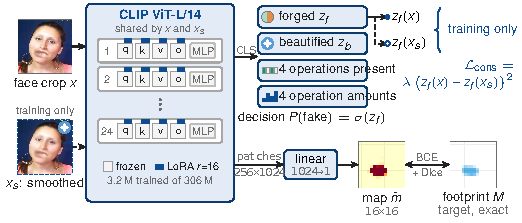
\includegraphics[width=\columnwidth]{figs_tikz/fig_arch_v7}
\caption{The model and the training rule. A frozen CLIP ViT-L/14 with rank-16 LoRA on the q, k, v and output projections
of all 24 blocks (3.2\,M of 306\,M parameters trained); linear heads on the CLS token give the forged logit $z_f$, the
beautified logit $z_b$ and four operation presence and quantity scores; a linear layer on the 256 patch tokens gives the
$16\times16$ evidence map $\hat m$, trained with BCE and Dice against the exact footprint $M$ of the edit. The forgery decision
reads $P(\text{fake})=\sigma(z_f)$ only. Training only: a skin-smoothed copy $x_s$ of every item, drawn by one operator for
every class, passes through the same network and $\mathcal{L}_\text{cons}=\lambda\,(z_f(x)-z_f(x_s))^2$ ties its forged logit
to the clean one (SIC, Sec.~\ref{sec:sic}). Example: a held-out part-level forgery (mouth of another identity) and its map.}
\label{fig:arch}
\end{figure}
\textbf{Training data.} Every edited training image has a pixel-aligned original $x_0$, so the footprint of the edit is
exact, $M(x)=\mathrm{dilate}_\rho(\mathbf{1}[\|x-x_0\|_\infty>\tau])$ with $\tau=6$ on 8-bit intensities. On FF++
c23~\cite{ffpp} (official split) each step draws, from a genuine frame $x_0$, a genuine item, a beautified item (one of four
landmark and skin operations at a random strength, one of 14 colour filters~\cite{pilgram} or a random colour grading) and a
forged item (a self-blend of $x_0$~\cite{sbi}, an observed FF++ forgery or a part-level forgery), the forged item beautified
with probability 0.5; forged items without landmarks receive skin smoothing as a whole-crop filter rather than the face-local
operation, an asymmetry whose effect Sec.~\ref{sec:chain} measures. The FF++-only arms use nothing else. The full-data models
add 7,831 FFHQ photographs~\cite{ffhq} and their renders by Tencent and Megvii~\cite{retouchingffhq}, sister services of the
test service, each render decomposed by optical flow and a photometric residual into single-operation components (supplement),
and 61,510 part-level forgeries that transplant the eyes, nose or mouth of another identity or regenerate the part with
Stable Diffusion inpainting.

\textbf{Model} (Fig.~\ref{fig:arch}). A frozen CLIP ViT-L/14~\cite{clip} with rank-16 LoRA~\cite{lora} on every attention
projection (3.2\,M of 306\,M parameters trained). Two linear heads on the pooled feature give the forged logit $z_f$ and the
beautified logit $z_b$, with $P(\text{fake})=\sigma(z_f)$; an operation-presence head and a $1\times1$ convolution on the
spatial tokens (the $16\times16$ evidence map $\hat m$) are trained against the operation labels and $M$ with BCE and Dice,
and the classifier does not read $\hat m$. The forgery decision is read from $z_f$ alone; the beautified class and the
operation scores are attributes reported separately. The forgery-head-only model keeps $z_f$ and nothing else on the same
data; it is the first row of every detection table because it is at or above the full model on every untreated source on
both seeds, while the shared beautified head costs reenactment (Sec.~\ref{sec:detect}). Training: 224\,px, AdamW at
$10^{-4}$, 8 epochs, 16 genuine bases per batch; checkpoints are chosen on validation data only (supplement).

\subsection{Smoothing-invariant consistency}
\label{sec:sic}
The sign of the error follows the class that receives smoothed views (Sec.~\ref{sec:exposure}) and the cue is the
skin-smoothing signature itself (Fig.~\ref{fig:bandenergy}); the rule follows from both. For every training item $x$,
genuine, beautified or forged, a smoothed copy $x_s$ is drawn by one operator with one distribution of strengths, so that no
class can learn the form of the smoothing as a label, and the forged logit of the copy is asked not to move:
\begin{equation}
\mathcal{L}=\mathcal{L}_\text{BCE}\big(z_f(x),y\big)+\mathcal{L}_\text{map}+\lambda\,\big(\operatorname{sg}[z_f(x)]-z_f(x_s)\big)^2,
\label{eq:sic}
\end{equation}
where $\operatorname{sg}$ stops the gradient: the clean logit is the target, only the smoothed view is pulled, and the clean
path is trained by the classification loss alone. The map target of $x_s$ is the footprint of $x$. The operator is face-local
bilateral smoothing inside the landmark hull at a random strength, or whole-crop bilateral smoothing where no landmarks are
carried; the median filter, the Gaussian blend, the commercial renders and the AR renders are never used in training. Generic
consistency does not reach this: CORE~\cite{core} ties representations across flips, rotations, Gaussian blur and JPEG
re-encoding and still scores a smoothed genuine face above its original in 97\% of pairs (Fig.~\ref{fig:teaser}). The bars for
the rule were written before training (supplement): false alarms at most 15\% on face-local and whole-crop smoothing and on
the commercial renders; a miss rise on smoothed forgeries at most 5 points above the arm without views; untreated video AUC on
Celeb-DF-v2 and DFD, Celeb-DF-B AUC and DF40 reenactment AUC within stated bands of the model without the rule; a $\lambda=0$
control; two seeds. Sec.~\ref{sec:sicres} reports what the rule reaches and what it costs.

% ----------------------------------------------------------------------------
\section{Results}
\label{sec:results}
\begin{table*}[t]
\centering
\caption{Both errors under one rule ($P(\text{fake})$, threshold at 5\% FPR on each source's untreated genuine frames).
Celeb-DF-B: AUC untreated, re-encoded (AUC$_c$) and beautified (AUC$_b$), AUC lost beyond re-encoding, rise in misses and in
false alarms under the preset minus the rise under re-encoding, and FA$_b$, the false-alarm rate on beautified genuine frames.
DFD: sixteen held-out filters on the full frame. Percentage points. Intervals, the Celeb-DF-v2 filter source and video-level
AUC in the supplement (Tables~\ref{S-tab:twosidedfull} and~\ref{S-tab:cdfbextra}). $^\ddagger$General generated-image detectors,
not trained on faces. $^\dagger$Trained on more data than the published detectors (supplement).}
\label{tab:twosided}
\scriptsize
\setlength{\tabcolsep}{3pt}
\begin{adjustbox}{max width=\textwidth}\begin{tabular}{@{}ll ccccccc cccc@{}}
\toprule
 & & \multicolumn{7}{c}{Celeb-DF-B, app presets (frame level)} & \multicolumn{4}{c}{DFD + 16 held-out filters (frame level)} \\
\cmidrule(lr){3-9}\cmidrule(lr){10-13}
Detector & train & AUC & AUC$_c$ & AUC$_b$ & AUC$_c{-}$AUC$_b$ & $\Delta$MISS$_\text{beauty}$ & FA$_b$ & $\Delta$FA$_\text{beauty}$ & AUC & AUC$_f$ & $\Delta$MISS & $\Delta$FA \\
\midrule
Xception~\cite{xception} & FF++ c23 & 0.811 & 0.795 & 0.737 & 0.058 & +10.9 & 5.7 & -1.7 & 0.854 & 0.834 & +2.0 & +2.0 \\
EfficientNet-B4~\cite{efficientnet} & FF++ c23 & 0.811 & 0.798 & 0.762 & 0.035 & +3.4 & 7.8 & +1.7 & 0.810 & 0.781 & +6.3 & -0.5 \\
F3Net~\cite{f3net} & FF++ c23 & 0.798 & 0.782 & 0.731 & 0.051 & +10.9 & 5.4 & -1.9 & 0.781 & 0.774 & -8.5 & +3.6 \\
SPSL~\cite{spsl} & FF++ c23 & 0.781 & 0.769 & 0.727 & 0.042 & +12.4 & 3.4 & -2.4 & 0.829 & 0.837 & +4.7 & -1.8 \\
UCF~\cite{ucf} & FF++ c23 & 0.841 & 0.829 & 0.777 & 0.053 & +11.3 & 5.7 & +0.2 & 0.822 & 0.804 & +5.0 & +0.3 \\
RECCE~\cite{recce} & FF++ c23 & 0.785 & 0.765 & 0.723 & 0.042 & +13.8 & 4.1 & -3.6 & 0.833 & 0.808 & +7.3 & -0.2 \\
CORE~\cite{core} & FF++ c23 & 0.821 & 0.808 & 0.752 & 0.057 & +13.5 & 4.0 & -2.2 & 0.827 & 0.821 & -5.4 & +1.6 \\
SRM~\cite{srm} & FF++ c23 & 0.789 & 0.769 & 0.733 & 0.035 & +15.3 & 2.8 & -3.4 & 0.830 & 0.822 & +5.8 & +0.2 \\
SBI~\cite{sbi} & FF++ c23 & 0.875 & 0.861 & 0.752 & 0.109 & +21.8 & 1.8 & -0.6 & 0.829 & 0.810 & +4.5 & +0.4 \\
UnivFD$^\ddagger$~\cite{univfd} & ProGAN$^\ddagger$ & 0.653 & 0.637 & 0.624 & 0.013 & -7.2 & 7.6 & +4.5 & 0.840 & 0.801 & -10.2 & +11.6 \\
NPR$^\ddagger$~\cite{npr} & ProGAN$^\ddagger$ & 0.503 & 0.503 & 0.498 & 0.006 & -0.7 & 3.4 & +0.9 & 0.473 & 0.516 & -13.7 & +9.4 \\
Effort~\cite{effort} & FF++ c23 & 0.909 & 0.882 & 0.807 & 0.075 & +11.0 & 5.4 & +2.1 & 0.939 & 0.905 & +15.1 & -2.3 \\
Forensics Adapter~\cite{forensicsadapter} & FF++ c23 & 0.909 & 0.894 & 0.828 & 0.066 & +15.2 & 7.9 & +0.1 & 0.940 & 0.924 & +8.0 & -0.6 \\
GenD~\cite{gend2026} & FF++ c23 & 0.924 & 0.898 & 0.807 & 0.091 & +12.0 & 9.9 & +3.6 & 0.934 & 0.925 & +3.1 & +1.2 \\
DFD-HR~\cite{dfdhr2026} & FF++ c23 & 0.938 & 0.915 & 0.838 & 0.077 & +3.6 & 14.6 & +9.8 & 0.943 & 0.928 & +9.1 & -2.0 \\
CADDM~\cite{caddm} & FF++ raw & 0.886 & 0.850 & 0.762 & 0.088 & -2.9 & 13.8 & +9.9 & 0.845 & 0.818 & +3.8 & +0.8 \\
LAA-Net~\cite{laanet} & FF++ raw & 0.889 & 0.870 & 0.698 & 0.172 & +14.7 & 6.0 & +3.3 & 0.810 & 0.783 & +6.2 & +0.0 \\
\midrule
P0 & FF++ & 0.927 & 0.901 & 0.860 & 0.041 & +17.0 & 5.1 & -1.6 & 0.943 & 0.924 & +9.3 & -0.2 \\
P2-sym & FF++ & 0.920 & 0.900 & 0.866 & 0.034 & +14.2 & 5.5 & -1.2 & 0.936 & 0.921 & +7.3 & -0.4 \\
\oursB{}$^\dagger$ & FF++, FFHQ & 0.949 & 0.934 & 0.896 & 0.038 & +7.0 & 7.4 & +2.3 & 0.961 & 0.952 & +4.2 & +0.2 \\
\quad second seed$^\dagger$ & FF++, FFHQ & 0.955 & 0.939 & 0.904 & 0.035 & +5.7 & 8.3 & +3.2 & 0.951 & 0.938 & +3.8 & +1.1 \\
\oursF{}$^\dagger$ & FF++, FFHQ & 0.938 & 0.918 & 0.866 & 0.052 & +6.7 & 9.5 & +4.9 & 0.942 & 0.931 & +8.9 & -1.0 \\
\quad second seed$^\dagger$ & FF++, FFHQ & 0.941 & 0.926 & 0.883 & 0.043 & +8.3 & 6.7 & +2.7 & 0.945 & 0.931 & +4.4 & +0.3 \\
\oursF{}, sym.\ view$^\dagger$ & FF++, FFHQ & 0.941 & 0.925 & 0.868 & 0.057 & +10.0 & 9.2 & +4.9 & 0.947 & 0.934 & +8.5 & -0.9 \\
\quad second seed$^\dagger$ & FF++, FFHQ & 0.945 & 0.934 & 0.888 & 0.046 & +3.1 & 8.7 & +4.9 & 0.954 & 0.940 & +2.6 & +2.9 \\
\bottomrule
\end{tabular}
\end{adjustbox}
\end{table*}

\begin{table}[t]
\centering
\caption{Commercial skin smoothing (Smoothing-90): 2,210 FFHQ originals and their renders. Share of renders scored above their
own original (50 means no shift), medians of $P(\text{fake})$, median paired shift of the forgery logit with a bootstrap
interval over originals, share of renders above the threshold that accuses 5\% of the originals, and share above the
threshold fixed on FF++ validation. NPR scores everything at 1.0.}
\label{tab:retouch}
\scriptsize
\setlength{\tabcolsep}{2pt}
\begin{adjustbox}{max width=\columnwidth}\begin{tabular}{@{}l ccccc@{}}
\toprule
Detector & above own orig.\ (\%) & median $P(\text{fake})$ & median $\Delta$logit [95\% CI] & accused (\%) & FF++-val.\ thr.\ (\%) \\
\midrule
Xception~\cite{xception} & 95.2 & 0.29 $\rightarrow$ 0.94 & +3.32 [+3.17, +3.45] & 51.6 & 65.0 \\
EfficientNet-B4~\cite{efficientnet} & 93.7 & 0.32 $\rightarrow$ 0.96 & +3.48 [+3.33, +3.57] & 36.3 & 63.8 \\
F3Net~\cite{f3net} & 97.8 & 0.13 $\rightarrow$ 0.97 & +4.92 [+4.74, +5.08] & 50.6 & 69.0 \\
SPSL~\cite{spsl} & 97.3 & 0.46 $\rightarrow$ 0.96 & +3.05 [+2.95, +3.12] & 51.2 & 56.3 \\
UCF~\cite{ucf} & 95.4 & 0.03 $\rightarrow$ 0.98 & +5.47 [+5.20, +5.73] & 41.4 & 48.4 \\
RECCE~\cite{recce} & 96.5 & 0.12 $\rightarrow$ 0.94 & +3.82 [+3.70, +3.96] & 36.8 & 60.0 \\
CORE~\cite{core} & 96.6 & 0.25 $\rightarrow$ 0.95 & +3.90 [+3.74, +4.03] & 54.8 & 66.7 \\
SRM~\cite{srm} & 99.3 & 0.46 $\rightarrow$ 0.67 & +0.68 [+0.65, +0.71] & 62.8 & 62.0 \\
SBI~\cite{sbi} & 96.2 & 0.21 $\rightarrow$ 0.99 & +4.88 [+4.72, +5.04] & 37.3 & 93.3 \\
UnivFD$^\ddagger$~\cite{univfd} & 90.4 & 0.01 $\rightarrow$ 0.02 & +1.22 [+1.17, +1.28] & 16.6 & 15.2 \\
NPR$^\ddagger$~\cite{npr} & n/a & n/a & n/a & n/a & n/a \\
Effort~\cite{effort} & 95.6 & 0.32 $\rightarrow$ 0.59 & +0.96 [+0.90, +1.02] & 43.2 & 31.1 \\
Forensics Adapter~\cite{forensicsadapter} & 93.3 & 0.06 $\rightarrow$ 0.35 & +1.72 [+1.59, +1.87] & 39.7 & 32.5 \\
GenD~\cite{gend2026} & 98.5 & 0.23 $\rightarrow$ 0.92 & +3.27 [+3.19, +3.35] & 68.7 & 67.4 \\
DFD-HR~\cite{dfdhr2026} & 99.0 & 0.21 $\rightarrow$ 0.71 & +2.06 [+1.93, +2.15] & 64.9 & 56.2 \\
CADDM~\cite{caddm} & 60.9 & 0.54 $\rightarrow$ 0.74 & +0.67 [+0.53, +0.81] & 6.3 & 42.3 \\
LAA-Net~\cite{laanet} & 89.2 & 0.23 $\rightarrow$ 0.97 & +3.60 [+3.36, +3.79] & 17.2 & 81.0 \\
\midrule
P0 & 98.5 & 0.05 $\rightarrow$ 0.97 & +5.17 [+5.05, +5.38] & 54.2 & -- \\
P2-sym & 53.7 & 0.02 $\rightarrow$ 0.02 & +0.09 [+0.03, +0.12] & 5.9 & -- \\
\oursB{}$^\dagger$ & 70.5 & 0.00 $\rightarrow$ 0.00 & +0.41 [+0.38, +0.44] & 9.1 & 0.2 \\
\quad second seed$^\dagger$ & 68.2 & 0.00 $\rightarrow$ 0.00 & +0.19 [+0.16, +0.19] & 6.5 & 0.1 \\
\oursF{}$^\dagger$ & 32.5 & 0.00 $\rightarrow$ 0.00 & -1.20 [-1.28, -1.12] & 8.6 & 0.5 \\
\oursF{}, sym.\ view$^\dagger$ & 30.0 & 0.00 $\rightarrow$ 0.00 & -1.09 [-1.19, -1.00] & 8.1 & 0.1 \\
\bottomrule
\end{tabular}
\end{adjustbox}
\end{table}

\begin{figure}[t]
\centering
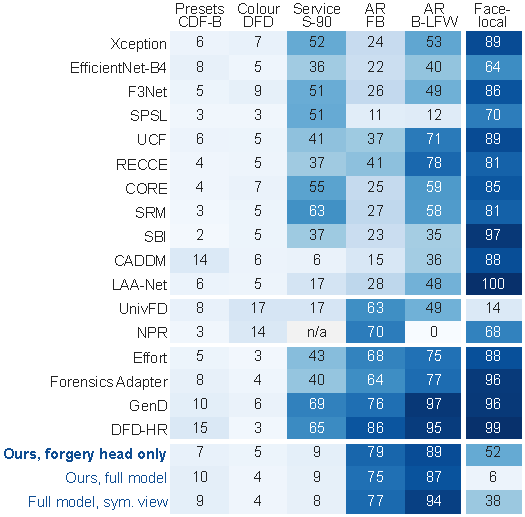
\includegraphics[width=\columnwidth]{fig_accuse_v6b}
\caption{Accused share of beautified genuine faces (\%) at the threshold that accuses 5\% of each source's untreated genuine
faces: Celeb-DF-B presets (FA$_b$), DFD under sixteen colour filters, commercial Smoothing-90, Instagram AR renders of
FairBeauty (FB) and B-LFW, and the scripted face-local smoothing of Celeb-DF-v2 genuine frames (strength 0.06). Rows: eleven
face-forgery CNNs, two general detectors, four CLIP detectors, and our full-data models (first seed). NPR is saturated on the
service.}
\label{fig:accuse}
\end{figure}

\subsection{Both errors under one rule}
\label{sec:accuse}
\label{sec:measure}
\textbf{Commercial retouching.} Table~\ref{tab:retouch} reads the Smoothing-90 renders against their own originals. Fifteen
of the seventeen detectors score the render above its original in 89--99\% of pairs, and the median $P(\text{fake})$ moves
from 0.21 to 0.99 for SBI and from 0.23 to 0.92 for GenD: a heavily smoothed genuine face is scored like a forgery whatever the
threshold (sign test $p<10^{-10}$ for every detector but NPR, whose scores saturate; CADDM 60.9\%). At the threshold that
accuses 5\% of the originals thirteen detectors accuse 36--69\% of the renders; with a threshold fixed on FF++ validation they
accuse 15--93\%, and three of them already call 31--45\% of the untouched originals fake (Table~\ref{S-tab:deploy}).
Whitening, face slimming and eye enlarging at their strongest level stay at 3.7--8.1\% for thirteen of the sixteen detectors
other than NPR (Table~\ref{S-tab:v4perop}); they pass through the same service, encoder and resolution, so the retouching
result is a smoothing result. Our full-data models accuse 6.5--12.5\% of the renders, but none leaves the score unmoved:
\oursB{} still ranks the render above its original in 68--71\% of pairs, and \oursF{} moves it the other way (below its
original in 67.5\%). They were trained on renders of the two sister services, which the published detectors were not.

\textbf{Skin-only smoothing.} A bilateral filter inside the face hull, background untouched, is accused by all seventeen
detectors (Fig.~\ref{fig:accuse}, Table~\ref{S-tab:smooth38}): the four CLIP detectors call 88--99\% of genuine frames forged at
the milder strength and 99.9--100\% at the stronger one, the eleven face-forgery CNNs 64--100\% and 92--100\%, UnivFD 14 and
55\%. At matched visible strength skin-only smoothing is accused more often than whole-crop smoothing.

\textbf{Instagram AR filters.} All seventeen detectors accuse FairBeauty renders above the 5\% floor (10.7--85.9\%) and sixteen
accuse B-LFW renders (12.0--96.6\%); every published detector ranks the render above its own original in 69--99\% of pairs
(Table~\ref{S-tab:ar}). Re-compressing both sides keeps 0.64--1.05 of each accused share, so re-compression does not carry the
effect, although the AR capture path stays confounded with the beautification. Our models are not exempt (\oursB{} 79--82\%
on FairBeauty, more than Effort and Forensics Adapter): our training removes the accusation on the vendor family it saw, not on
AR filters.

\textbf{App presets.} On Celeb-DF-B every detector that detects the untreated forgeries loses frame AUC beyond what
re-encoding costs (Table~\ref{tab:twosided}): SBI 0.861 to 0.752, CADDM 0.850 to 0.762, LAA-Net 0.870 to 0.698, and
0.066--0.091 for the four CLIP detectors; at video level CADDM goes from 0.965 to 0.832, against 0.91 to 0.76 reported by
Libourel et al.~\cite{libourel2024}. Beyond re-encoding the presets raise the miss rate by 11--22 points (SBI, Effort,
Forensics Adapter, GenD, LAA-Net) and false alarms by 4--10 points (GenD, CADDM, DFD-HR); under the DFD filters Effort's miss
rate rises by 15.1 points and Forensics Adapter's by 8.0.

\subsection{Dose response}
\begin{figure}[t]
\centering
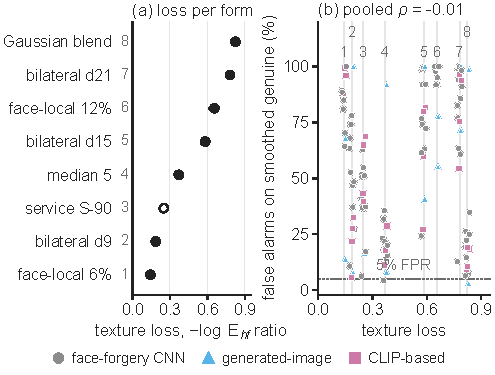
\includegraphics[width=\columnwidth]{fig_bandenergy}
\caption{The shared cue is the beautification signature, not blur. (a) Texture loss of eight smoothing forms, measured as the
high-frequency energy removed inside the face hull of 400 genuine Celeb-DF-v2 frames (commercial Smoothing-90 on 200 FFHQ
pairs, hollow). (b) False-alarm rate of each published detector at each form against that loss: pooled Spearman $-0.01$.
A Gaussian blend removes the most energy and is accused least; a face-local bilateral filter removes less and is accused by
nearly every detector. Matched contrasts and the per-band scan are in the supplement.}
\label{fig:bandenergy}
\end{figure}

\label{sec:mechanism}
On the 1,348 genuine Celeb-DF-v2 frames we varied the strength of three edits and read the forgery logit of the four released
CLIP detectors (Table~\ref{S-tab:dose}). Under face-local smoothing the logit rises in at least 97.9\% of frames at every level
for all four and the median shift grows with strength: the weakest level already moves it by 1.0--1.9 times the gap between
the detector's mean forged and mean genuine logit, the strongest by 1.9--3.0 gaps. Whole-crop bilateral smoothing gives the
same picture at smaller shifts. A radial vignette alone does not: three of the four move the other way. For the published
CLIP detectors smoothing is the operative edit, and a genuine face is pushed past the forged mean.

\textbf{The cue is the beautification signature.} If the detectors reacted to lost texture, forms that remove more
high-frequency energy would be accused more. They are not (Fig.~\ref{fig:bandenergy}): on 400 genuine frames the energy above
0.25 cycles per pixel lost inside the face hull ranges from 0.19 (face-local 0.06) to 0.94 (Gaussian blend, whole-crop
bilateral 21), and the false-alarm rate of the seventeen detectors across the seven forms does not follow it (pooled Spearman
$+0.06$). What it follows is the beautification signature: with the same kernel, confining the smoothing to the face raises the
accusation by 28 points (16 of 17 detectors, $p=5\times10^{-4}$); at equal energy loss an edge-preserving filter is accused 67
points more than a uniform blur (16 of 17); and only the band 0.02--0.12 cycles per pixel, the skin relief that a bilateral
filter flattens and a Gaussian blend leaves, correlates with the accusation ($\rho=+0.45$). The detectors respond to flattened
skin with kept edges inside the face, which a beautification filter produces and a forgery boundary or a generator leaves
behind, not to blur as such. This is why Gaussian blur or JPEG as a training view does not remove the accusation
(Sec.~\ref{sec:chain}) and why the operator of Sec.~\ref{sec:sic} is skin smoothing.

\subsection{Which class receives beautified views}
\label{sec:exposure}
\begin{figure}[t]
\centering
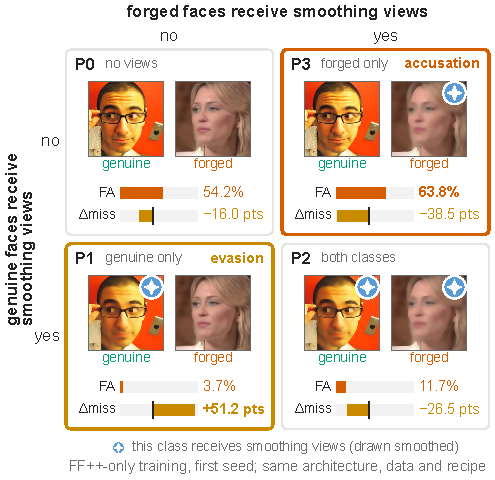
\includegraphics[width=\columnwidth]{fig_exposure_v7}
\caption{The class that receives smoothed training views decides the direction of the error. FF++-only arms with the same architecture,
data and recipe, first seed (Table~\ref{S-tab:tradeofffull}). FA: commercial Smoothing-90 renders accused at the threshold that
accuses 5\% of their originals. $\Delta$miss: change of the miss rate on Celeb-DF-v2 forgeries under strong whole-crop
smoothing at the same rule; a negative change means the arm accuses every smoothed face. Thumbnails show the training views
each class receives; a badge marks a class that receives smoothed views. P1 opens an evasion route; P3 accuses.}
\label{fig:exposure}
\end{figure}
With architecture, data and recipe fixed, P0--P3 differ only in which class receives beautified views
(Fig.~\ref{fig:exposure}; arm definitions in the supplement). On Celeb-DF-B the beautification-specific miss rise is
11--17 points for P0 (three seeds), 20--22 for P1 and 10--13 for P2; P1 exceeds P0 by 4.5--9.5 points in every seed
(Holm-adjusted $p\le0.01$), while P2 against P0 changes sign within the seed spread (Table~\ref{S-tab:exposure}). The
forged-only arm P3 (one seed, pre-declared reading) mirrors P1: it accuses 63.8\% of the Smoothing-90 renders ($+9.6$ over P0)
and 98--100\% of smoothed genuine frames, catches smoothed forgeries more often than untreated ones, and accuses 47\% of filtered
Celeb-DF-v2 genuine frames against 19\% for P0 (Table~\ref{S-tab:p3}). The sign rule holds: genuine-only views lower the
accusation and open evasion, forged-only views raise the accusation and close evasion, and views on both classes sit in between.
Exposure moves errors between misses and false alarms; it does not make the classes more separable (P3 untreated Celeb-DF-v2
video AUC 0.943 against 0.938 for P0). P0 already keeps more AUC under the presets (0.86--0.88) than released Effort (0.81), so
most of the margin of our models over the CLIP baselines comes from the base recipe, not from exposure.

\subsection{Smoothing views: what the exposure arms taught}
\label{sec:chain}
The FF++-only arms with pre-registered bars give three findings (supplement Sec.~\ref{S-sec:chain},
Table~\ref{S-tab:tradeofffull}). No other view substitutes for smoothing. P0 accuses 44--56\% of the Smoothing-90
renders although it trains with label-symmetric blur, rescaling and JPEG, and removing smoothing from the beautified views
(P2-nosmooth) brings the accusation back to 55--67\%. Genuine-only smoothing views are an evasion route. P1-smooth
accuses 0.7--1.0\% of the renders and then misses 96--100\% of bilaterally smoothed forgeries on frames it has never seen
(a miss rise of 56--63 points), 75--84\% of median-filtered ones and 51--54\% of blended ones; it has learnt that smoothed means
genuine. A class-asymmetric form is learnt as a label. When genuine items receive face-local smoothing and forged items
a whole-crop filter, a whole-crop filter on a genuine frame is called forged in 35--90\% of frames by \oursF{}, against
1--40\% for P0. Drawing one form for both classes (P2-sym) removes the whole-crop accusation (false alarms 2--6\%) but not
the skin-only one (38--99\%), and under Effort's tuning scheme it meets only one of its two bars. These limits are what the
constraint of Sec.~\ref{sec:sic} addresses.

\subsection{Removing the cue: SIC}
\label{sec:sicres}
\begin{table*}[t]
\centering
\caption{Smoothing-invariant consistency against the model trained without it (forgery head only, same data, views, seeds
and checkpoint rule). FA: smoothed genuine Celeb-DF-v2 frames called fake at the 5\%-FPR rule (face-local 0.06 / 0.12, whole-crop
bilateral 15); S-90: commercial Smoothing-90 renders accused at the threshold of their originals; $\Delta$miss: miss rise on
face-local 0.12 smoothed forgeries; untreated video AUC on Celeb-DF-v2 and DFD; Celeb-DF-B AUC; DF40 reenactment video AUC
(FF++ identities); bars passed of the six pre-registered bars. Seed 1 and 2 where both were trained.}
\label{tab:sic}
\footnotesize
\begin{tabular}{@{}lcccccccccccc@{}}
\toprule
Model & seed & \multicolumn{3}{c}{smoothed genuine accused (\%)} & S-90 & $\Delta$miss & \multicolumn{2}{c}{untreated video AUC} & Celeb-DF-B & DF40 FR & bars \\
 & & fl 0.06 & fl 0.12 & bil 15 & acc.\ \% & fl 0.12 & CDFv2 & DFD & AUC & ff & passed \\
\midrule
forgery head only, no rule & 1 & 51.6 & 84.5 & 35.5 & 9.1 & $-$34.0 & 0.956 & 0.987 & 0.866 & 0.842 & -- \\
\midrule
symmetric view only ($\lambda=0$) & 1 & 53.9 & 91.8 & 1.6 & 11.9 & $-$40.1 & 0.943 & 0.975 & 0.891 & 0.835 & 3/6 \\
SIC, $\lambda=0.03$ & 1 & 5.0 & 3.3 & 9.6 & 11.2 & 24.4 & 0.946 & 0.979 & 0.886 & 0.750 & 4/6 \\
SIC, $\lambda=0.03$ & 2 & 3.8 & 3.5 & 8.8 & 15.0 & 20.4 & 0.933 & 0.975 & 0.876 & 0.777 & 2/6 \\
SIC, $\lambda=0.1$ & 1 & 6.5 & 4.2 & 9.9 & 10.5 & 15.8 & 0.930 & 0.980 & 0.871 & 0.774 & 3/6 \\
SIC, $\lambda=0.1$ & 2 & 4.6 & 4.6 & 8.5 & 8.1 & 17.6 & 0.929 & 0.974 & 0.868 & 0.771 & 2/6 \\
SIC, $\lambda=0.3$ & 1 & 6.0 & 4.2 & 8.1 & 12.8 & 9.5 & 0.898 & 0.971 & 0.840 & 0.692 & 2/6 \\
SIC, $\lambda=1$ & 1 & 5.8 & 4.4 & 5.8 & 2.1 & 9.7 & 0.907 & 0.986 & 0.835 & 0.768 & 2/6 \\
SIC, $\lambda=1$ & 2 & 6.2 & 5.5 & 6.3 & 12.3 & 6.1 & 0.844 & 0.968 & 0.804 & 0.746 & 2/6 \\
one-sided penalty & 1 & 0.1 & 0.1 & 0.0 & 9.2 & 56.5 & 0.954 & 0.980 & 0.880 & 0.794 & 4/6 \\
one-sided penalty & 2 & 0.1 & 0.0 & 0.0 & 10.4 & 47.3 & 0.929 & 0.975 & 0.860 & 0.775 & 2/6 \\
Gaussian view (ablation) & 1 & 5.8 & 19.5 & 1.1 & 3.5 & $-$13.5 & 0.855 & 0.971 & 0.819 & 0.782 & 1/6 \\
Gaussian view (ablation) & 2 & 5.9 & 14.5 & 1.3 & 8.7 & $-$9.3 & 0.848 & 0.960 & 0.821 & 0.784 & 2/6 \\
SIC, $\lambda=1$, FF++ only & 1 & 7.4 & 6.8 & 5.3 & 7.0 & 4.8 & 0.856 & 0.979 & 0.829 & 0.674 & 2/6 \\
\bottomrule
\end{tabular}

\end{table*}
\begin{figure}[t]
\centering
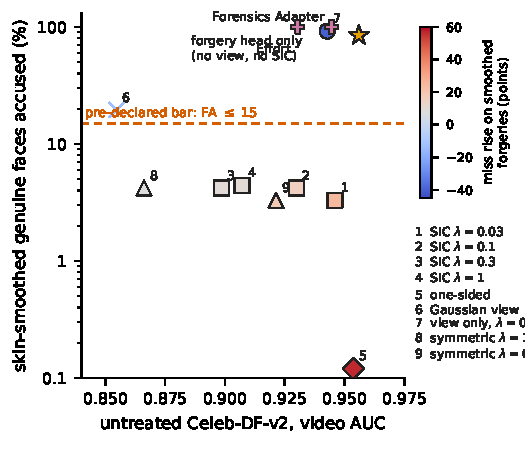
\includegraphics[width=\columnwidth]{fig_sic_curve}
\caption{The trade-off traced by the SIC family. Each point is one trained model: untreated Celeb-DF-v2 video AUC against the
share of skin-smoothed genuine faces accused (face-local 0.12, log scale); colour gives the rise of the miss rate on the same
smoothing applied to forgeries. The star is the model without the rule; crosses are Effort and Forensics Adapter. Every
penalty weight removes the accusation; smaller weights keep untreated detection and let more smoothed forgeries through;
the one-sided penalty keeps everything except the forgeries. The Gaussian view fails the accusation bar.}
\label{fig:siccurve}
\end{figure}
\textbf{Three ways not to remove the cue.} A fixed threshold accuses smoothed genuine faces (Sec.~\ref{sec:accuse}).
Raising the threshold with a smoothing estimate does not help either: with the full model's smoothing-presence output as
the covariate and the shift learnt on FF++ validation genuine renders only, the accusation of strongly smoothed genuine
faces falls to 0--1\% for Effort, Forensics Adapter, DFD-HR and our model, and 78--100\% of the smoothed forgeries now pass,
because the two score distributions coincide (AUC between smoothed genuine and smoothed forged faces 0.60--0.66 for the four
CLIP detectors; supplement). Changing the weights with a view on genuine faces only removes the accusation and opens the
evasion route (Sec.~\ref{sec:exposure}). What remains is a view on both classes with a constraint on the forgery logit.

\textbf{What the constraint buys and costs.} Table~\ref{tab:sic} and Fig.~\ref{fig:siccurve} give the family. The
symmetric view alone ($\lambda=0$) leaves detection untouched and the accusation in place (54 / 92\% at the two face-local
strengths), so the consistency term, not the view, removes the accusation; every $\lambda\ge0.03$ does so (3--7\%). The term
also sets the cost, and the cost has two faces. With the gradient through both sides at $\lambda=1$ the clean forgery score is
pulled toward its smoothed copy and untreated detection falls (Celeb-DF-v2 0.866, in-domain forgery recall 90.9 to 69.8\%);
the stop-gradient halves that loss (0.907) and smaller weights shrink it further (0.930 at 0.1, 0.946 at 0.03), but as
$\lambda$ falls the smoothed forgery's score falls with the genuine one and its miss rises ($+10$, $+16$, $+24$ points). The
one-sided penalty, which forbids a rise of the forgery logit under smoothing and allows a fall, is the limit of that
direction: untreated AUC 0.954, accusation 0.1\%, and 57 points more smoothed forgeries missed. DF40 reenactment is 0.06--0.09
below the model without the rule at every weight (its seed spread is 0.014), the one bar no member passes. A Gaussian blur
of the same spatial support in place of the skin-smoothing operator fails the accusation bar at the strong face-local form
(19.5\%) and opens the bilateral evasion ($+14$ to $+22$ points): the operator has to be the beautification signature.
Trained on FF++ alone, the rule still removes the accusation (5--7\%), so the effect does not depend on our added data.
Instagram AR renders stay accused (SIC 67.7\%, Effort 67.8\%; Sec.~\ref{sec:limits}). Under smoothing of both classes the SIC
models keep an AUC of 0.77--0.78 at the strong face-local form against 0.60--0.66 for the published CLIP detectors
(supplement): the separation that a threshold cannot recover is kept, at the price above.

\subsection{Untreated detection and DF40}
\label{sec:detect}
\textbf{Celeb-DF-v2 and DFD.} Each baseline is scored on its own crop and our models on ours (Table~\ref{S-tab:reproduce}).
\oursB{} reaches a frame AUC of 0.914 on Celeb-DF-v2 and 0.961 on DFD (second seed 0.923 and 0.951): above Effort on both
sets, above all four CLIP detectors on DFD, and on par with Forensics Adapter and GenD on Celeb-DF-v2 (paired intervals). Under
the app presets it keeps 0.896 and 0.904 against 0.807--0.838 for the four CLIP detectors, every paired interval above zero
under video and identity resampling (Table~\ref{S-tab:cdfbpaired}); the equal-data arm P0 is 0.022--0.053 above them as well.
Identity resampling changes 24 of 563 intervals, none of them a headline (Table~\ref{S-tab:identity}).

\textbf{Forgery head only against the full model.} On the same data \oursB{} is above \oursF{} on Celeb-DF-v2 frames
($+0.023$, $+0.036$), on Celeb-DF-B under the presets ($+0.030$, $+0.021$) and most on DF40 reenactment ($+0.076$ to $+0.145$),
every interval above zero on both seeds: the shared beautified head costs detection.

\textbf{DF40} (Table~\ref{S-tab:v4df40full}). On the nine face-swap methods \oursB{} is on par with GenD, at or above Effort and
Forensics Adapter, and 0.012--0.024 behind DFD-HR. On the twelve reenactment methods it is 0.076--0.094 behind GenD and DFD-HR in
the FF++ domain and 0.13--0.18 behind GenD in the Celeb-DF domain, on par with Effort and Forensics Adapter; every SIC member
is a further 0.06--0.09 below (Sec.~\ref{sec:sicres}). Across the published detectors the share of smoothed renders ranked
above their original does not predict reenactment AUC ($\rho=0.36$, $p=0.23$), so we claim no link beyond our arms. On six
entire-face synthesis methods our models are below Effort and GenD on every method (Table~\ref{S-tab:efs}), and the three-way
model sends 42--89\% of ddim and SiT stills to \emph{beautified}: smooth synthesised skin is absorbed by that class.

\subsection{Localisation and restoration of part-level forgeries}
\label{sec:cgd}
For a detected part-level forgery with footprint $M$, let $\hat A$ be the $|M|$ highest cells of $\hat m$ and
$x_A=x\odot(1-A)+x_0\odot A$ restore region $A$ to the original. These results are those of the evidence head of \oursF{} (the
forgery-head-only model has none); it reaches
IoU$_7$ (IoU with the footprint on a $7\times7$ grid) of 0.83--0.84 on three held-out editors (SDXL never used in training),
and restoring the region it names removes 93.5--94.0\% of its detections against 93.6--94.1\% for the true footprint
(Table~\ref{S-tab:cgd_all}; second seed 90.2--90.9\% against 90.2--91.0\%). Restoring the complement removes at most 0.4\%, a
centred region 39--41\%; post-hoc maps without the head reach IoU$_7$ 0.33--0.41. Any accurate segmenter of the edit would score
similarly, so the test does not show the classifier's reasoning, and it does not cover whole-face swaps or accused genuine faces.

\subsection{What did not work}
\label{sec:negative}
Under pre-registered bars (Sec.~\ref{S-sec:negative}): adversarial or random training over a measured beautification operator
(seven variants) stays within $\pm$0.01 AUC of colour grading and loses 0.02--0.05 untreated AUC; a learned inverse of the edit
does not lower false alarms; a decision pooled from the evidence map halves false alarms under filters and lets 7.5 points more
beautified forgeries through; fine-tuning released Effort with beautified views moves its operating point, not its AUC; fusion
with CADDM still ranks smoothed renders above their originals in 87--92\% of pairs (Sec.~\ref{S-sec:fusion}).

% ----------------------------------------------------------------------------
\section{Limitations}
\label{sec:limits}
The measurement covers four app presets, 27 colour filters, eight AR filters on two face sets and one retouching service that
became an analysis set; a fresh smoothing source is needed, and the AR capture path is confounded with the beautification. The
class boundary is stated, not measured. P3 and the one-sided, Gaussian and $\lambda=0.03$ arms have one seed, and no non-CLIP
pipeline was trained with the rule. Our models accuse AR renders as much as the published CLIP detectors (\oursB{} 79--90\%,
SIC 68\%), so the rule removes the accusation for the smoothing family it was drawn from, not for beautification in general.
\oursB{} is behind GenD and DFD-HR on DF40 reenactment and every SIC member is a further 0.06--0.09 below; the full model's
beautified head costs detection and sends 21\% of the service's originals to the beautified class. Effort and DFD-HR were not
reproduced at their published numbers, DFDC is not evaluated, and inference cost was not measured.

\section{Conclusion}
Seventeen published detectors share one failure. They rank a skin-smoothed genuine face above its own original because the detectors respond to flattened skin with kept edges, which beautification produces and forgery leaves
behind. The failure comes from training. Which class receives smoothed views decides whether the error is an accusation or an
evasion, and genuine-only views open an evasion route. It cannot be removed at the threshold, because the smoothed scores of genuine and forged faces
coincide. A class-symmetric smoothing view with a consistency term on the forgery logit keeps the separation under smoothing
and removes the accusation, and we report what that costs along the penalty weight: untreated detection at large weights,
misses on smoothed forgeries at small ones, and reenactment at every weight. The sources, the rule and the paired reader are
released so that the next detector can be read the same way.

\bibliographystyle{IEEEtran}
\bibliography{refs_v6}
\end{document}
